% !TEX TS-program = pdflatex
% !TEX root = ../tesi.tex

%************************************************
\chapter{Introduction}
\label{chp:intro}
%************************************************

Imagine a third dimension with it's own interactive coherence with physical laws foreign for us. Denaturalization, an expanded virtual environment. But why should we have to understand this complex dimension, if we have not yet learned about the one in which we live?
Yet we strive to do it, every day.

\begin{flushright}
	\itshape
	Thus, guided by algorithms, the human being increasingly loses his power to act, his autonomy. \\
	He finds himself faced with a world that escapes his understanding. \\
	He sticks to algorithmic decisions that he cannot fully understand, algorithms become black boxes.\\
	\medskip
	--- Byung-Chul Han, "The not-things", 2022
\end{flushright}

My work is a new immersive approach to the electroacoustic composition based on a interactive abstraction integrated in the sound design of a video game.
The music, the sound design, the evocation of physical and emotional perceptions given by sound feedback. With these tools we are able to connect with any dimension we want.
With my work I want to provide not only an interactive approach to electroacoustic composition, but also to provide to the user an immersive experience in a dimension that works at deep levels of \textbf{abstraction} and \textbf{denaturalization}: a virtual reality in which every gesture of the player is linked to a non-traditional sound feedback.
What makes the workflow interactive? The composition exercise is based on the generation of interpolated samples of organic objects and sounds generated with additive, subtractive, granular and modular synthesis - which modulation parameters change randomly in real time - whenever an action is performed inside the game. The result is the generation of different electroacoustic gestures which, interacting each other, generate an electro-acoustic composition that always sounds different, for the randomness of the actions and the non-linearity of the game's events.
All the samples are electroacoustic gestures made by computational music algorithm written in \textbf{Wolfram language}. The codes are computed in a computing environment called \textbf{Mathematica}

\begin{comment}
\begin{code}
\documentclass[\meta{\dots\unkern}]{scrreprt} % or scrbook or scrartcl

\usepackage[\meta{\dots\unkern}]{classicthesis}
\usepackage{arsclassica}

\begin{document}
\dots
\end{document}
\end{code}

For example, this document has been produced with the following code:
\begin{code}
\documentclass[a4paper,twoside,openright,titlepage,
               headinclude,footinclude,BCOR5mm,
               numbers=noenddot,cleardoublepage=empty,
               tablecaptionabove]{scrreprt}

\usepackage{\meta{\dots\unkern}}
\usepackage{subfig}
\usepackage[eulerchapternumbers,subfig,beramono,eulermath,pdfspacing]%
           {classicthesis}
\usepackage{arsclassica}

\begin{document}
\dots
\end{document}
\end{code}

It is recommended to use the \optname{beramono} and \optname{eulerchapternumbers} options together with \arsclassica.



\section{Style}

The typographical style achieved with \arsclassica{} differs from \classicthesis{} in the following points:
\begin{itemize}
\item use of Iwona font, by Janusz Nowacki, for the sectioning unit titles (chapters, sections, subsections, sub-subsections, paragraphs and subparagraphs), for the description list labels, the headlines and the caption labels (\classicthesis{} doesn't use any sans serif font);
\item customized chapter numbers;
\item semi-transparent headlines; the headlines are separated from the page number by a small rule;
\item caption labels in boldface (\classicthesis{} doesn't use any boldface font);
\item itemize lists with semi-transparent bullets.
\end{itemize}

\arsclassica{} is designed  to provide a ready-to-use typographical style: for this reason it has no loading options and it is \emph{not} configurable or customizable in any way. If you change the previous settings, you'll risk to destroy the balance of the style, so it is \emph{highly recommended} to keep them unchanged.

One of the principles of \LaTeX{} is that it allows the author to take no interest in the typographical questions, permitting him to focus only on the structure and the contents of his document. This fact should always be kept in mind: using a style written by others, the user accepts all the typographical settings chosen for him by the author of the style, and he isn't forced to study typography to fine-tune the layout of his publications. This is the case of \arsclassica{} too: if you change its settings, you'll deny this philosophy and, consequently, you'll have to study (a lot of) typography to achieve acceptable results.

The style achieved with \arsclassica{} is \emph{not} therefore configurable or customizable. The typographical style is very personal: if you like this package and find attractive the idea to take no interest in the problem of the style definition, then you'll use \arsclassica{} with satisfaction; otherwise, if you have different needs or you aren't satisfied with the layout of the package, then you should try other classes or packages, even building your own style.



\section{Important}

To write a document according to the \arsclassica{} style, you have to follow some very simple rules.
\begin{itemize}
\item Don't change \emph{for any reason} the \arsclassica{} settings (fonts, text body size, colors, \dots).
\item The sectioning unit titles (chapters, section, subsections, \dots) have to be \emph{one line long}, possibly in \emph{plain text} (no symbols, formulas or code fragments). If you have titles longer than one line, try and rephrase them: you can almost always do it.
\item In the table of contents and in the list of tables and figures, captions have to be \emph{one line long}, possibly in \emph{plain text}. Use the optional argument of sectioning commands and of \cmdname{caption}, if necessary.
\item Don't use \optname{tocaligned} and \optname{dottedtoc} options of \classicthesis: the default table of contents does the job very well (see the documentation of \classicthesis{} for a nice discussion of this point).
\item Don't use vertical or double rules in your tables (see the documentation of \pkgname{booktabs}).
\item Use footnotes and margin notes very sparingly.
\item If your document includes graphs and plots, draw them using \LaTeX{} (by \pkgname{Ti\emph{k}Z} and \pkgname{pgfplots}, for example) and not an external software. This is the only way to get the best typographical outcome.
\end{itemize}
\end{comment}



%\section{Examples}
%intendo sostituire queste immagini con qualcuna inerente al mio progetto
\begin{figure}
\centering
\subfloat[Asia personas duo]
{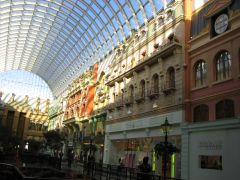
\includegraphics[width=.45\columnwidth]{Lorem}} \quad
\subfloat[Pan ma signo]
{\label{fig:example-b}%
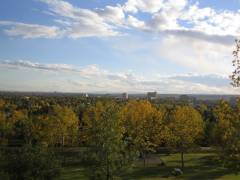
\includegraphics[width=.45\columnwidth]{Ipsum}} \\
\subfloat[Methodicamente o uno]
{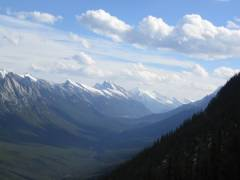
\includegraphics[width=.45\columnwidth]{Dolor}} \quad
\subfloat[Titulo debitas]
{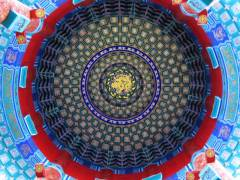
\includegraphics[width=.45\columnwidth]{Sit}}
\caption[Tu duo titulo debitas latente]{Tu duo titulo debitas latente}
\label{fig:example}
\end{figure}

\begin{comment}Please note that the content of this section is just some dummy text. It isn't a real language.

Lorem ipsum dolor sit amet, consectetuer adipiscing elit. Ut purus elit, vestibulum ut, placerat ac, adipiscing vitae, felis. Curabitur dictum gravida mauris.

\subsection*{A subsection}

\lipsum[2]

\subsubsection*{A sub-subsection}

\lipsum[7]

\paragraph{A paragraph}
Lorem ipsum dolor sit amet, consectetuer adipiscing elit. Ut purus elit, vestibulum ut, placerat ac, adipiscing vitae, felis. Curabitur dictum gravida mauris. Nam arcu libero, nonummy eget, consectetuer id, vulputate a, magna.

\paragraph{Another paragraph}
Cras nec ante, pellentesque a nulla, cum sociis natoque penatibus et magnis dis parturient montes, nascetur ridiculus mus. Aliquam tincidunt urna

\bigskip

Donec aliquet, tortor sed accumsan bibendum, erat ligula aliquet magna, vitae ornare odio metus a mi. Morbi ac orci et nisl hendrerit mollis. Suspendisse ut massa. Cras nec ante. Pellentesque a nulla. Cum sociis natoque penatibus et magnis dis parturient montes, nascetur ridiculus mus. Aliquam tincidunt urna.

\begin{description}
\item[Mane] Lorem ipsum dolor sit amet, consectetuer adipiscing elit.
\item[Tekel] Ut purus elit, vestibulum ut, placerat ac, adipiscing vitae, felis. Curabitur dictum gravida mauris.
\item[Fares] Nam arcu libero, nonummy eget, consectetuer
id, vulputate a, magna.
\end{description}

\begin{table}
\caption{Lorem ipsum dolor sit amet}
\centering
\begin{tabular}{ll}
\toprule
\textbf{Alkaloid} & \textbf{Origin} \\
\midrule
atropine & belladonna \\
morphine & poppy \\
nicotine & tobacco \\
\bottomrule
\end{tabular}
\end{table}

Suspendisse vel felis. Ut lorem lorem, interdum eu, tincidunt sit amet, laoreet vitae, arcu. Aenean faucibus pede eu ante. Praesent enim elit, rutrum at, molestie non, nonummy vel, nisl. Ut lectus eros, malesuada sit amet, fermentum eu, sodales cursus, magna. Donec eu purus. Quisque vehicula, urna sed ultricies auctor, pede lorem egestas dui, et convallis elit erat sed nulla.

\subsection*{Some formulas}

Una formula in linea viene incorporata nel testo: $\lim_{n \to \infty}\sum_{k=1}^n \frac{1}{k^2} = \frac{\pi^2}{6}$, per esempio. Come si osserva, \LaTeX{} fa \emph{il possibile} per comprimerla e modificare il meno possibile l'interlinea nel capoverso che la contiene.
Una formula in display viene invece composta da \LaTeX{} su linee a parte, separate dal contesto con adeguati spazi bianchi per metterla in mostra e farla risaltare sulla pagina.
\begin{equation}
\lim_{n \to \infty}\sum_{k=1}^n \frac{1}{k^2}= \frac{\pi^2}{6}
\end{equation}
Come si osserva, ora la formula risulta centrata, non compressa, e tutti i suoi elementi occupano il giusto spazio con un risultato finale di grande respiro.

Integer tempus convallis augue. Etiam facilisis. Nunc elementum fermentum wisi. Aenean placerat. Ut imperdiet, enim sed gravida sollicitudin, felis odio placerat quam, ac pulvinar elit purus eget enim.

\begin{equation}
\int_a^{a+T}f(x)\,dx= \int_0^T f(x)\,dx
\qquad
\oint f(z)\,dz=2\pi i
\end{equation}

Nulla malesuada porttitor diam. Donec felis erat, congue non, volutpat at, tincidunt tristique, libero. Vivamus viverra fermentum felis. Donec non- ummy pellentesque ante.

\begin{equation}
f(x_1,\dots,x_n)=  \prod_{k=1}^n x_k
\qquad
\sum_{k=1}^n x_k^2=1
\qquad
\biggl(\sum_n x_n^2\biggr)^{1/2}
\end{equation}

\lipsum[2]

\begin{equation}
\begin{bmatrix}
a_{11} & \dots & a_{1n} \\
a_{21} & \dots & a_{2n} \\
\hdotsfor{3} \\
a_{n1} & \dots & a_{nn}
\end{bmatrix}
\end{equation}

\lipsum[4]

\begin{equation}
\lim_{x\to 0}
\frac{\sin x}{x}=1 \qquad
\lim_{n\to +\infty}f_n=\delta
\end{equation}

Fusce mauris. Vestibulum luctus nibh at lectus. Sed bibendum, nulla a faucibus semper, leo velit ultricies tellus, ac venenatis arcu wisi vel nisl. Vestibulum diam.

\begin{equation}
n!=
\begin{cases}
1       & \text{if $n=0$} \\
n(n-1)! & \text{if $n\ge 1$}
\end{cases}
\end{equation}

Ut lectus eros, malesuada sit amet, fermentum eu, sodales cursus, magna. Donec eu purus. Quisque vehicula, urna sed ultricies auctor, pede lorem egestas dui, et convallis elit erat sed nulla. Donec luctus. Curabitur et nunc. Aliquam dolor odio, commodo pretium, ultricies non, pharetra in, velit.

\begin{equation}
x_G=
\frac{\displaystyle
      \sum_{i=1}^n m_ix_i}
{\displaystyle\sum_{i=1}^n m_i}
\end{equation}

\lipsum[6]

\begin{equation}
\kappa =\frac{\xi}{E_{\textrm{max}}}
\qquad
E_{\textup{max}} =\frac{2 m_{\textup{e}} \beta^2\gamma^2 }{1 +2\gamma m_{\textup{e}}/m_{\textrm{x}} + ( m_{\textup{e}}/m_{\textup{x}})^2}
\end{equation}

\lipsum[8]
\end{comment}